\documentclass{article}

\usepackage{fancyhdr}
\usepackage{extramarks}
\usepackage{amsmath,mathrsfs,amssymb}
\usepackage{amsthm}
\usepackage{amsfonts}
\usepackage{tikz}
\usepackage[plain]{algorithm}
\usepackage{algpseudocode}
\usepackage[]{mcode}
\usepackage{graphicx}
\usepackage{pgfplots}
\usepackage{xfrac,siunitx}
\usepackage{gensymb}
\usepackage{caption}
\usepackage{epstopdf}

\usetikzlibrary{automata,positioning}

%
% Basic Document Settings
%

\topmargin=-0.45in
\evensidemargin=0in
\oddsidemargin=0in
\textwidth=6.5in
\textheight=9.0in
\headsep=0.25in

\linespread{1.1}

\pagestyle{fancy}
\lhead{\hmwkAuthorName}
\chead{\hmwkClass\ (\hmwkClassInstructor\ \hmwkClassTime): \hmwkTitle}
\rhead{\firstxmark}
\lfoot{\lastxmark}
\cfoot{\thepage}

\renewcommand\headrulewidth{0.4pt}
\renewcommand\footrulewidth{0.4pt}

\setlength\parindent{0pt}

%
% Create Problem Sections
%

\newcommand{\enterProblemHeader}[1]{
    \nobreak\extramarks{}{Problem \arabic{#1} continued on next page\ldots}\nobreak{}
    \nobreak\extramarks{Problem \arabic{#1} (continued)}{Problem \arabic{#1} continued on next page\ldots}\nobreak{}
}

\newcommand{\exitProblemHeader}[1]{
    \nobreak\extramarks{Problem \arabic{#1} (continued)}{Problem \arabic{#1} continued on next page\ldots}\nobreak{}
    \stepcounter{#1}
    \nobreak\extramarks{Problem \arabic{#1}}{}\nobreak{}
}

\setcounter{secnumdepth}{0}
\newcounter{partCounter}
\newcounter{homeworkProblemCounter}
\setcounter{homeworkProblemCounter}{1}
\nobreak\extramarks{Problem \arabic{homeworkProblemCounter}}{}\nobreak{}

%
% Homework Problem Environment
%
% This environment takes an optional argument. When given, it will adjust the
% problem counter. This is useful for when the problems given for your
% assignment aren't sequential. See the last 3 problems of this template for an
% example.
%
\newenvironment{homeworkProblem}[1][-1]{
    \ifnum#1>0
        \setcounter{homeworkProblemCounter}{#1}
    \fi
    \section{Problem \arabic{homeworkProblemCounter}}
    \setcounter{partCounter}{1}
    \enterProblemHeader{homeworkProblemCounter}
}{
    \exitProblemHeader{homeworkProblemCounter}
}

%
% Homework Details
%   - Title
%   - Due date
%   - Class
%   - Section/Time
%   - Instructor
%   - Author
%

\newcommand{\hmwkTitle}{Tutorial\ 1}
\newcommand{\hmwkDueDate}{July 25, 2016}
\newcommand{\hmwkClass}{Control Engineering}
\newcommand{\hmwkClassTime}{}
\newcommand{\hmwkClassInstructor}{Professor Friso De Boer}
\newcommand{\hmwkAuthorName}{S.Reynolds (262538)}

%
% Title Page
%

\title{
    \vspace{2in}
    \textmd{\textbf{\hmwkClass:\ \hmwkTitle}}\\
    \normalsize\vspace{0.1in}\small{Due\ on\ \hmwkDueDate\ at 3:00pm}\\
    \vspace{0.1in}\large{\textit{\hmwkClassInstructor\ \hmwkClassTime}}
    \vspace{3in}
}

\author{\textbf{\hmwkAuthorName}}
\date{}

\renewcommand{\part}[1]{\textbf{\large Part \Alph{partCounter}}\stepcounter{partCounter}\\}

%
% Various Helper Commands
%

% Useful for algorithms
\newcommand{\alg}[1]{\textsc{\bfseries \footnotesize #1}}

% For derivatives
\newcommand{\deriv}[1]{\frac{\mathrm{d}}{\mathrm{d}x} (#1)}

% For partial derivatives
\newcommand{\pderiv}[2]{\frac{\partial}{\partial #1} (#2)}

% Integral dx
\newcommand{\dx}{\mathrm{d}x}

% Alias for the Solution section header
\newcommand{\solution}{\textbf{\large Solution}}

% Probability commands: Expectation, Variance, Covariance, Bias
\newcommand{\E}{\mathrm{E}}
\newcommand{\Var}{\mathrm{Var}}
\newcommand{\Cov}{\mathrm{Cov}}
\newcommand{\Bias}{\mathrm{Bias}}

\DeclareMathOperator{\sinc}{sinc}

\begin{document}

\maketitle

\pagebreak

%%%%%%%%%%%%%%%%%%%%%%%%%%%%%%%%%%%%%%%%%%%%%%%%%%%%%%%%%%%%%%%%%%%%%%%%%%%%%%%%%%%%%%%%%%%%%%%%%%%%%%%%%%%%%%%%%%%%%%
% Question 1.1
%%%%%%%%%%%%%%%%%%%%%%%%%%%%%%%%%%%%%%%%%%%%%%%%%%%%%%%%%%%%%%%%%%%%%%%%%%%%%%%%%%%%%%%%%%%%%%%%%%%%%%%%%%%%%%%%%%%%%% 


    \textbf{Question 1.1}\\
    
    The selected .wav file was of a monkey, not music. The sample was a 16-bit sample which was 1.7 seconds in length, with a sampling frequency of 44100 $\si{\hertz}$. The code used to pre-process the file can be seen below:
    
    \begin{lstlisting}
	    % Clear all variables in the workspace and clear the screen
	    clear; clc; clf;
	    
	    % Create the file path to pass to wavread
	    file_name_1 = 'C:\Users\Shane Reynolds\Google Drive\University\';
	    file_name_2 = 'Charles Darwin University\Control Systems\Tutorial_1\';
	    file_name_3 = 'monkey2.wav';
	    
	    file_name = strcat(file_name_1,file_name_2,file_name_3);
	    
	    % Load the .wav file into u, with fs as teh sampling frequency and
	    % bits as the number of bits for the sample
	    [u,fs,bits]=wavread(file_name);
	    
	    % Split the channels from the original file into right and left
	    % signals
	    uleft = u(:,1);
	    uright = u(:,2);
	    
	    % To obtain a uniform time vector for the sample the sampling period
	    % was found and linspace used to create a time vector
	    Ts = 1/fs;
	    total_time = length(u)*Ts;
	    time = linspace(0,total_time,length(u))';
	    
	    % We wanted a slice of the sound file from 1.0s to 1.1s for analysis
	    % the code here represents the start and finish indexes for this time
	    % period
	    start_ind = 1/Ts;
	    finish_ind = 1.1/Ts;
	    
	    % Using the time indexes from above, samples from 1.0s to 1.1s for the
	    % left and right channels were obtained
	    sample_time_interval = time(start_ind:finish_ind,1);
	    sample_uleft = uleft(start_ind:finish_ind,1);
	    sample_uright = uright(start_ind:finish_ind,1);
	    
	    % Code plots the samples from the left and right channels for the
	    % time slice 1.0s to 1.1s
	    subplot(1,2,1)
	    plot(sample_time_interval,sample_uleft)
	    axis([1 1.1 -0.25 0.25]);
	    title('Left Channnel')
	    xlabel('time')
	    ylabel('magnitude')
	    
	    subplot(1,2,2)
	    plot(sample_time_interval,sample_uright)
	    axis([1 1.1 -0.25 0.25]);
	    title('Right Channnel')
	    xlabel('time')
	    ylabel('magnitude')
	    
	    % Print the range of the left and right channels to the console
	    fprintf('The range of the left channel is: %2.2d to %2.2d\n', ...
	    min(sample_uleft), max(sample_uleft))
	    fprintf('The range of the right channel is: %2.2d to %2.2d\n', ...
	    min(sample_uright), max(sample_uright))
    \end{lstlisting}
    
    \begin{figure}[H]
    	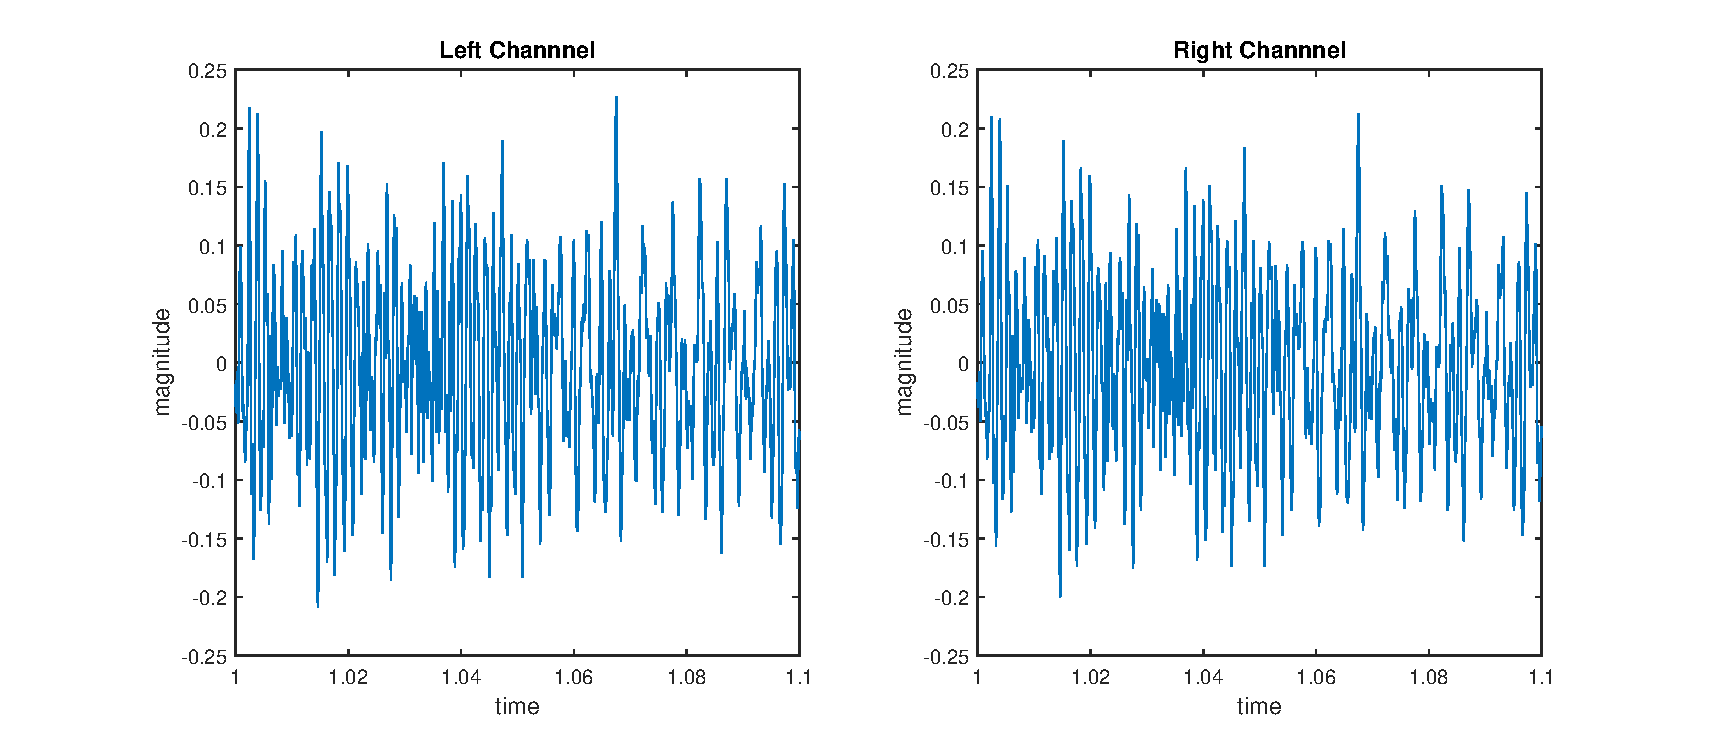
\includegraphics[scale=0.6]{fig1.eps}
    	\captionof{figure}{Time series plot of left and right stereo channels from 1.0s to 1.1s.}
    \end{figure}
    
    The time series plot for the left and right channels of the signal can be seen in Figure 1. The range of the amplitude from the left channel was -0.208 to 0.228. The range of the amplitude from the right channel was -0.201 to 0.212.\\



%%%%%%%%%%%%%%%%%%%%%%%%%%%%%%%%%%%%%%%%%%%%%%%%%%%%%%%%%%%%%%%%%%%%%%%%%%%%%%%%%%%%%%%%%%%%%%%%%%%%%%%%%%%%%%%%%%%%%%
% Question 1.3
%%%%%%%%%%%%%%%%%%%%%%%%%%%%%%%%%%%%%%%%%%%%%%%%%%%%%%%%%%%%%%%%%%%%%%%%%%%%%%%%%%%%%%%%%%%%%%%%%%%%%%%%%%%%%%%%%%%%%%


    
    \textbf{Question 1.3}\\
    
    The signal was to be filtered with a first order low pass filter, $G(s)$, which has a DC gain of 6$\si{\decibel}$, and a phase of -26.6$\si{\degree}$ at the frequency 250$\si{\hertz}$. A first order filter, according to Riedel (2015), is of the form:
    \begin{align}
	    G(s) = \frac{K_{DC}}{\tau s +1}
    \end{align}
    
    The parameter $K_{DC}$ in equation (1) refers to the DC gain and the parameter $\tau$ refers to the time constant. We know the DC gain and converting this from decibel, we can find this parameter. The following relationship links the magnitude to the magnitude expressed in decibels:
    \begin{align*}
	    K\si{\decibel} = 20 \log_{10}K_{DC}
    \end{align*}
    
    Rearranging and evaluating we get the following:
    \begin{align*}
	    K_{DC} 	&= 10^{\sfrac{K\si{\decibel}}{20}}\\
			    &= 10^{\sfrac{6}{20}}\\
			    &= 1.995
    \end{align*}
    
    Now, we simply need to find the time constant $\tau$. To do this we take advantage of the fact that we know a point on the phase plot. The phase of the filter, $G(s)$, is given by the following:
    \begin{align*}
	    \angle G(s) = \arctan \bigg(\frac{Im\{G(s)\}}{Re\{G(s)\}}\bigg)
    \end{align*}
	
	Letting $s = j \omega$, then we get:
	\begin{align}
	G(j \omega) = \frac{K_{DC}}{\tau j \omega +1}
	\end{align}
	
	Multiplying equation (2) by 1 (written using its complex conjugate), $\sfrac{1 - j \tau \omega}{1 - j \tau \omega}$, will give us:
	\begin{align*}
		G(j \omega) = \frac{K_{DC}}{1+(\tau \omega)^2} - j\frac{K_{DC} \tau \omega}{1+(\tau \omega)^2}
	\end{align*}
	
	We can now obtain an expression for $\angle G(j \omega)$, as follows:
	\begin{align*}
		\angle G(j \omega) = \arctan \bigg(-\frac{K_{DC} \cdot \tau \omega}{K_{DC}}\bigg)
	\end{align*}
	
	Rearranging, we can derive and expression for our time constant, $\tau$:
	\begin{align*}
		\tau 	&= -\frac{1}{\omega} \cdot \tan (\angle G(j \omega)) = -\frac{1}{2 \pi \cdot 250} \cdot \tan (-26.6) = \frac{1}{2 \pi \cdot 250} \cdot \tan (26.6)\\
				&= 3.18 \times 10^{-4} \ \si{\second.\per\radian}
	\end{align*}
	
	Hence, the transfer function for the lowpass filter is given by:
	
	\begin{align}
		G(s) = \frac{1.995}{(3.18 \times 10^{-4}) \cdot s + 1}
	\end{align}



%%%%%%%%%%%%%%%%%%%%%%%%%%%%%%%%%%%%%%%%%%%%%%%%%%%%%%%%%%%%%%%%%%%%%%%%%%%%%%%%%%%%%%%%%%%%%%%%%%%%%%%%%%%%%%%%%%%%%%
% Question 1.4
%%%%%%%%%%%%%%%%%%%%%%%%%%%%%%%%%%%%%%%%%%%%%%%%%%%%%%%%%%%%%%%%%%%%%%%%%%%%%%%%%%%%%%%%%%%%%%%%%%%%%%%%%%%%%%%%%%%%%%


    
    \textbf{Question 1.4}\\
    
    The bandwidth of a low pass filter is the corner frequency $\omega_c$, which can be found simply by taking the inverse of the time constant, $\tau$. That is:
    \begin{align*}
	    \omega_c 	&= \frac{1}{\tau} = \frac{1}{3.18 \times 10^{-4}}\\
				    &= 3144.65 \ \si{\radian.\per\second}
    \end{align*}
    	




%%%%%%%%%%%%%%%%%%%%%%%%%%%%%%%%%%%%%%%%%%%%%%%%%%%%%%%%%%%%%%%%%%%%%%%%%%%%%%%%%%%%%%%%%%%%%%%%%%%%%%%%%%%%%%%%%%%%%%
% Question 1.5
%%%%%%%%%%%%%%%%%%%%%%%%%%%%%%%%%%%%%%%%%%%%%%%%%%%%%%%%%%%%%%%%%%%%%%%%%%%%%%%%%%%%%%%%%%%%%%%%%%%%%%%%%%%%%%%%%%%%%%


    
    \textbf{Question 1.5}\\
    
    The following code was used to create a bode plot of the transfer function:
    
    \begin{lstlisting}
	    % Clear variables in the workspace, clear the screen and clear the
	    % present figures
	    clear; clc; clf;
	    
	    % Specify the variables for the transfer function
	    k_dc = 1.995;
	    Tc = 3.18e-4;
	    
	    % Create a symbolic representation of the transfer function G(s)
	    s = tf('s');
	    G = k_dc/(Tc*s + 1);
	    
	    % Create a Bode plot of the transfer function and plot the phase
	    % point that was given as a check for accuracy
	    hold on
	    bode(G)
	    plot(2*pi*250,-26.6,'ro')
    \end{lstlisting}
    
    The bode plot of the transfer function can be seen in Figure 2. From the top graph, the static frequency appears to be 6$\si{\decibel}$, and the phase at 250$\si{\hertz}$ can be seen to be approximately -26.6$\si{\degree}$ (as indicated by the red marker on the phase plot).
    
    \begin{figure}[H]
    	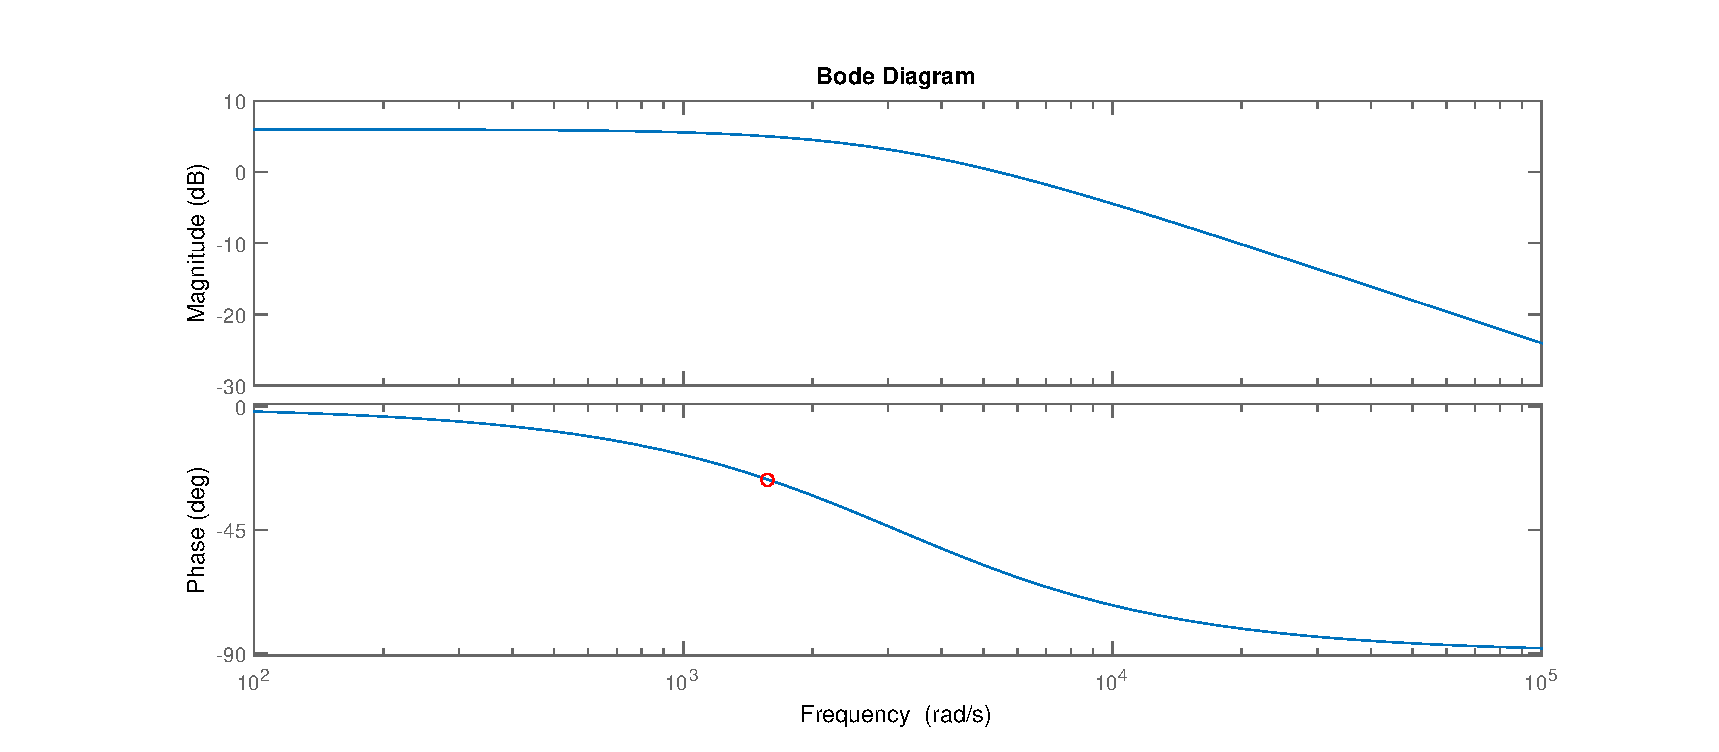
\includegraphics[scale=0.6]{fig2.eps}
    	\captionof{figure}{Bode plot showing both magnitude in decibels and phase in degrees.}
    \end{figure}
    

%%%%%%%%%%%%%%%%%%%%%%%%%%%%%%%%%%%%%%%%%%%%%%%%%%%%%%%%%%%%%%%%%%%%%%%%%%%%%%%%%%%%%%%%%%%%%%%%%%%%%%%%%%%%%%%%%%%%%%
% Question 1.6
%%%%%%%%%%%%%%%%%%%%%%%%%%%%%%%%%%%%%%%%%%%%%%%%%%%%%%%%%%%%%%%%%%%%%%%%%%%%%%%%%%%%%%%%%%%%%%%%%%%%%%%%%%%%%%%%%%%%%%
	
	\textbf{Question 1.6}\\
	
    The left and right signals were passed through the filter. The plotted results of the filtered and unfiltered channels can be seen in Figure 3.
    
    \begin{figure}[H]
    	\centering
    	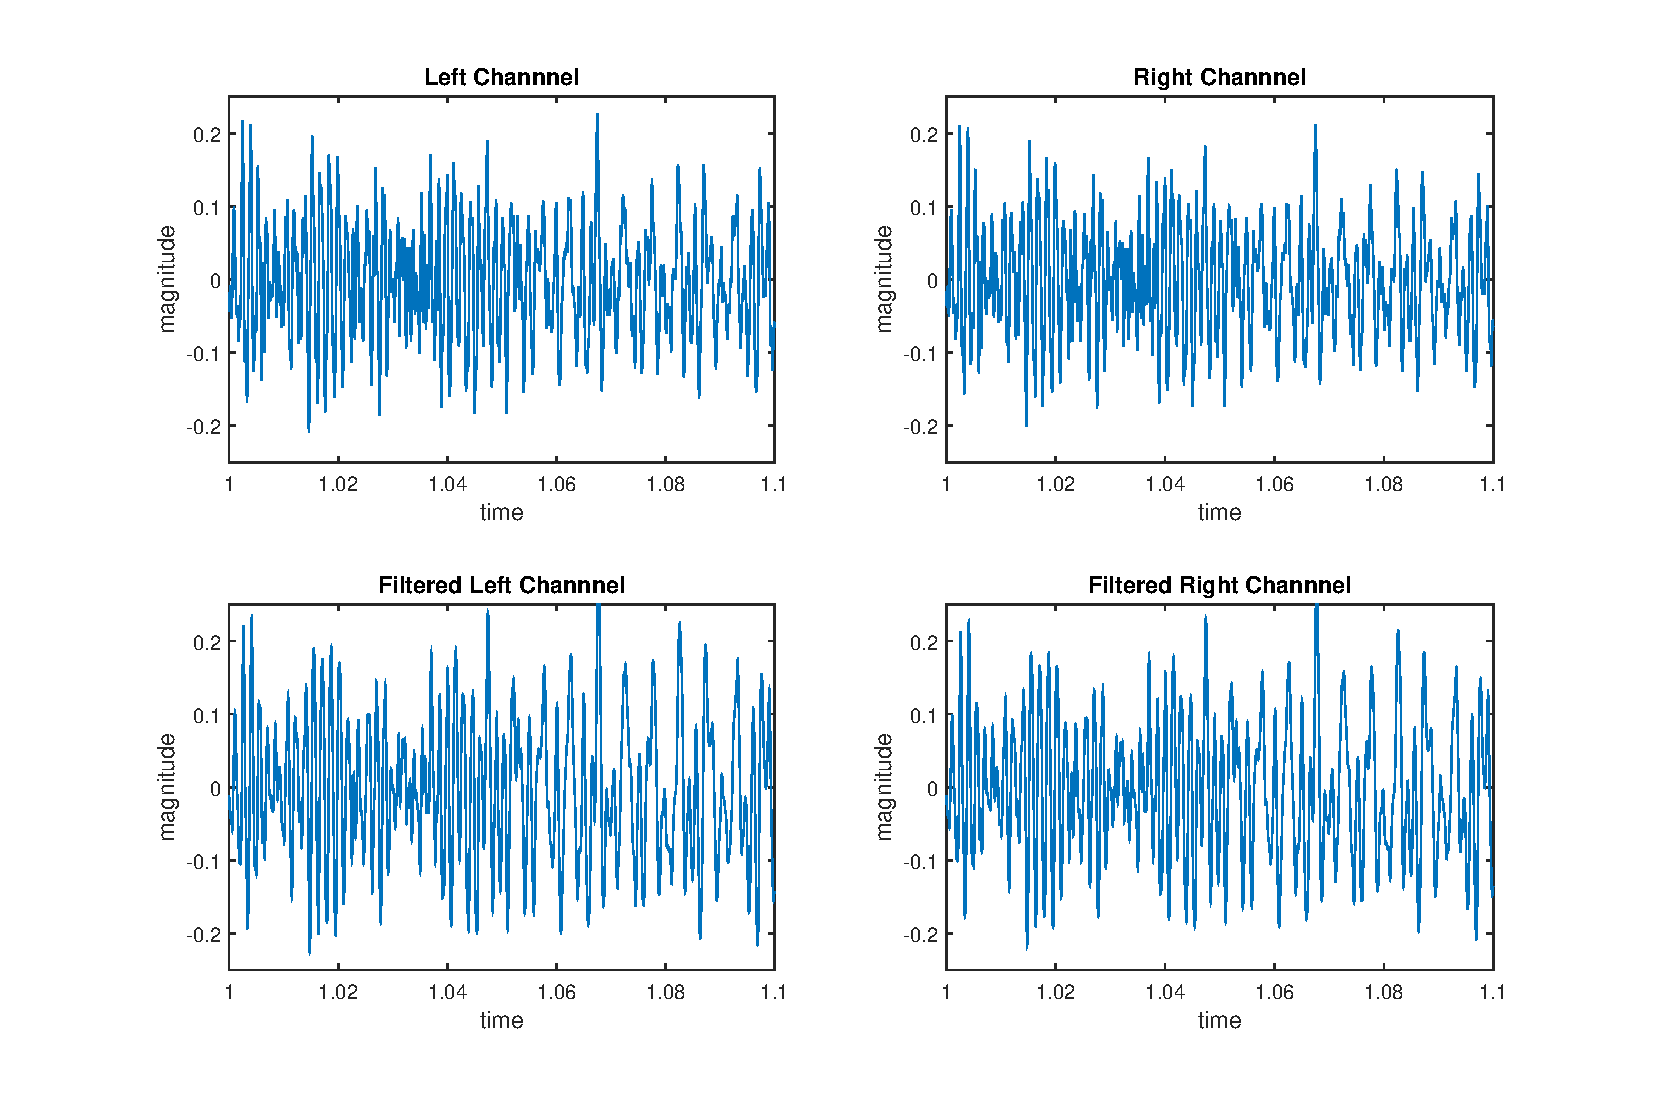
\includegraphics[scale=0.52]{fig3.eps}
    	\captionof{figure}{Bode plot showing both magnitude in decibels and phase in degrees.}
    \end{figure}
    
    	When the filtered sound was played and compared to the original sample, it was noticeably flatter. Specifically, the white noise hiss that often accompanies low quality field recordings was removed from the sample. Although the effect is not dramatic, evidence of the removal of high frequency hiss can be seen in Figure 3 - the filtered signals appear smoother. The plots were created using the code from question 1.1 plus the additional following code appended to the end:
    
    \begin{lstlisting}
	    % Pass both signals through the transfer function
	    sys = tf(1.995, [3.18e-4 1]);
	    yleft = lsim(sys,uleft,time);
	    yright = lsim(sys,uright,time);
	    
	    % Using the time indexes from above, samples from 1.0s to 1.1s for the
	    % left and right channels were obtained
	    sample_time_interval = time(start_ind:finish_ind,1);
	    sample_uleft = uleft(start_ind:finish_ind,1);
	    sample_uright = uright(start_ind:finish_ind,1);
	    
	    % Using the time indexes from above, samples from 1.0s to 1.1s for the
	    % left and right filtered channels were obtained
	    sample_yleft = yleft(start_ind:finish_ind,1);
	    sample_yright = yright(start_ind:finish_ind,1);
	    
	    % Code plots the samples and the filtered samples from the left 
	    % and right channels for the time slice 1.0s to 1.1s
	    subplot(2,2,1)
	    plot(sample_time_interval,sample_uleft)
	    axis([1 1.1 -0.25 0.25]);
	    title('Left Channnel')
	    xlabel('time')
	    ylabel('magnitude')
	    
	    subplot(2,2,2)
	    plot(sample_time_interval,sample_uright)
	    axis([1 1.1 -0.25 0.25]);
	    title('Right Channnel')
	    xlabel('time')
	    ylabel('magnitude')
	    
	    subplot(2,2,3)
	    plot(sample_time_interval,sample_yleft)
	    axis([1 1.1 -0.25 0.25]);
	    title('Filtered Left Channnel')
	    xlabel('time')
	    ylabel('magnitude')
	    
	    subplot(2,2,4)
	    plot(sample_time_interval,sample_yright)
	    axis([1 1.1 -0.25 0.25]);
	    title('Filtered Right Channnel')
	    xlabel('time')
	    ylabel('magnitude')
    \end{lstlisting}
	
	\newpage
	
%%%%%%%%%%%%%%%%%%%%%%%%%%%%%%%%%%%%%%%%%%%%%%%%%%%%%%%%%%%%%%%%%%%%%%%%%%%%%%%%%%%%%%%%%%%%%%%%%%%%%%%%%%%%%%%%%%%%%%
% Question 1.7
%%%%%%%%%%%%%%%%%%%%%%%%%%%%%%%%%%%%%%%%%%%%%%%%%%%%%%%%%%%%%%%%%%%%%%%%%%%%%%%%%%%%%%%%%%%%%%%%%%%%%%%%%%%%%%%%%%%%%%

	\textbf{Question 1.7}\\
	
	The original signals and the filtered signals were converted to their frequency domains using the Fast Fourier Transform. Figure 4 shows the plots of signal magnitude against their frequency in radians per second. This picture shows marginal amplification of the low frequency components in both the left and right channels. There is a much more dramatic attenuation of the signal for frequencies in the higher range. The plot shows frequencies all the way up to about 15000 $\si{\hertz}$ (approximately 100000 $\si{\radian.\per\second}$), which is nearing the end of the human audible range.\\
	
	The plots shown in Figure 4 confirm that there is dramatic attenuation of the high frequency components. In the Bode plot, we can see that unity amplification occurs at around 5000 $\si{\radian.\per\second}$ and continues until about 10000 $\si{\radian.\per\second}$. Signal attenuation is at a much higher level on the Bode plot as the frequency increases to about 11000 $\si{\radian.\per\second}$ and beyond. 
	
	 \begin{figure}[H]
	 	\hspace*{-1.5cm}
	 	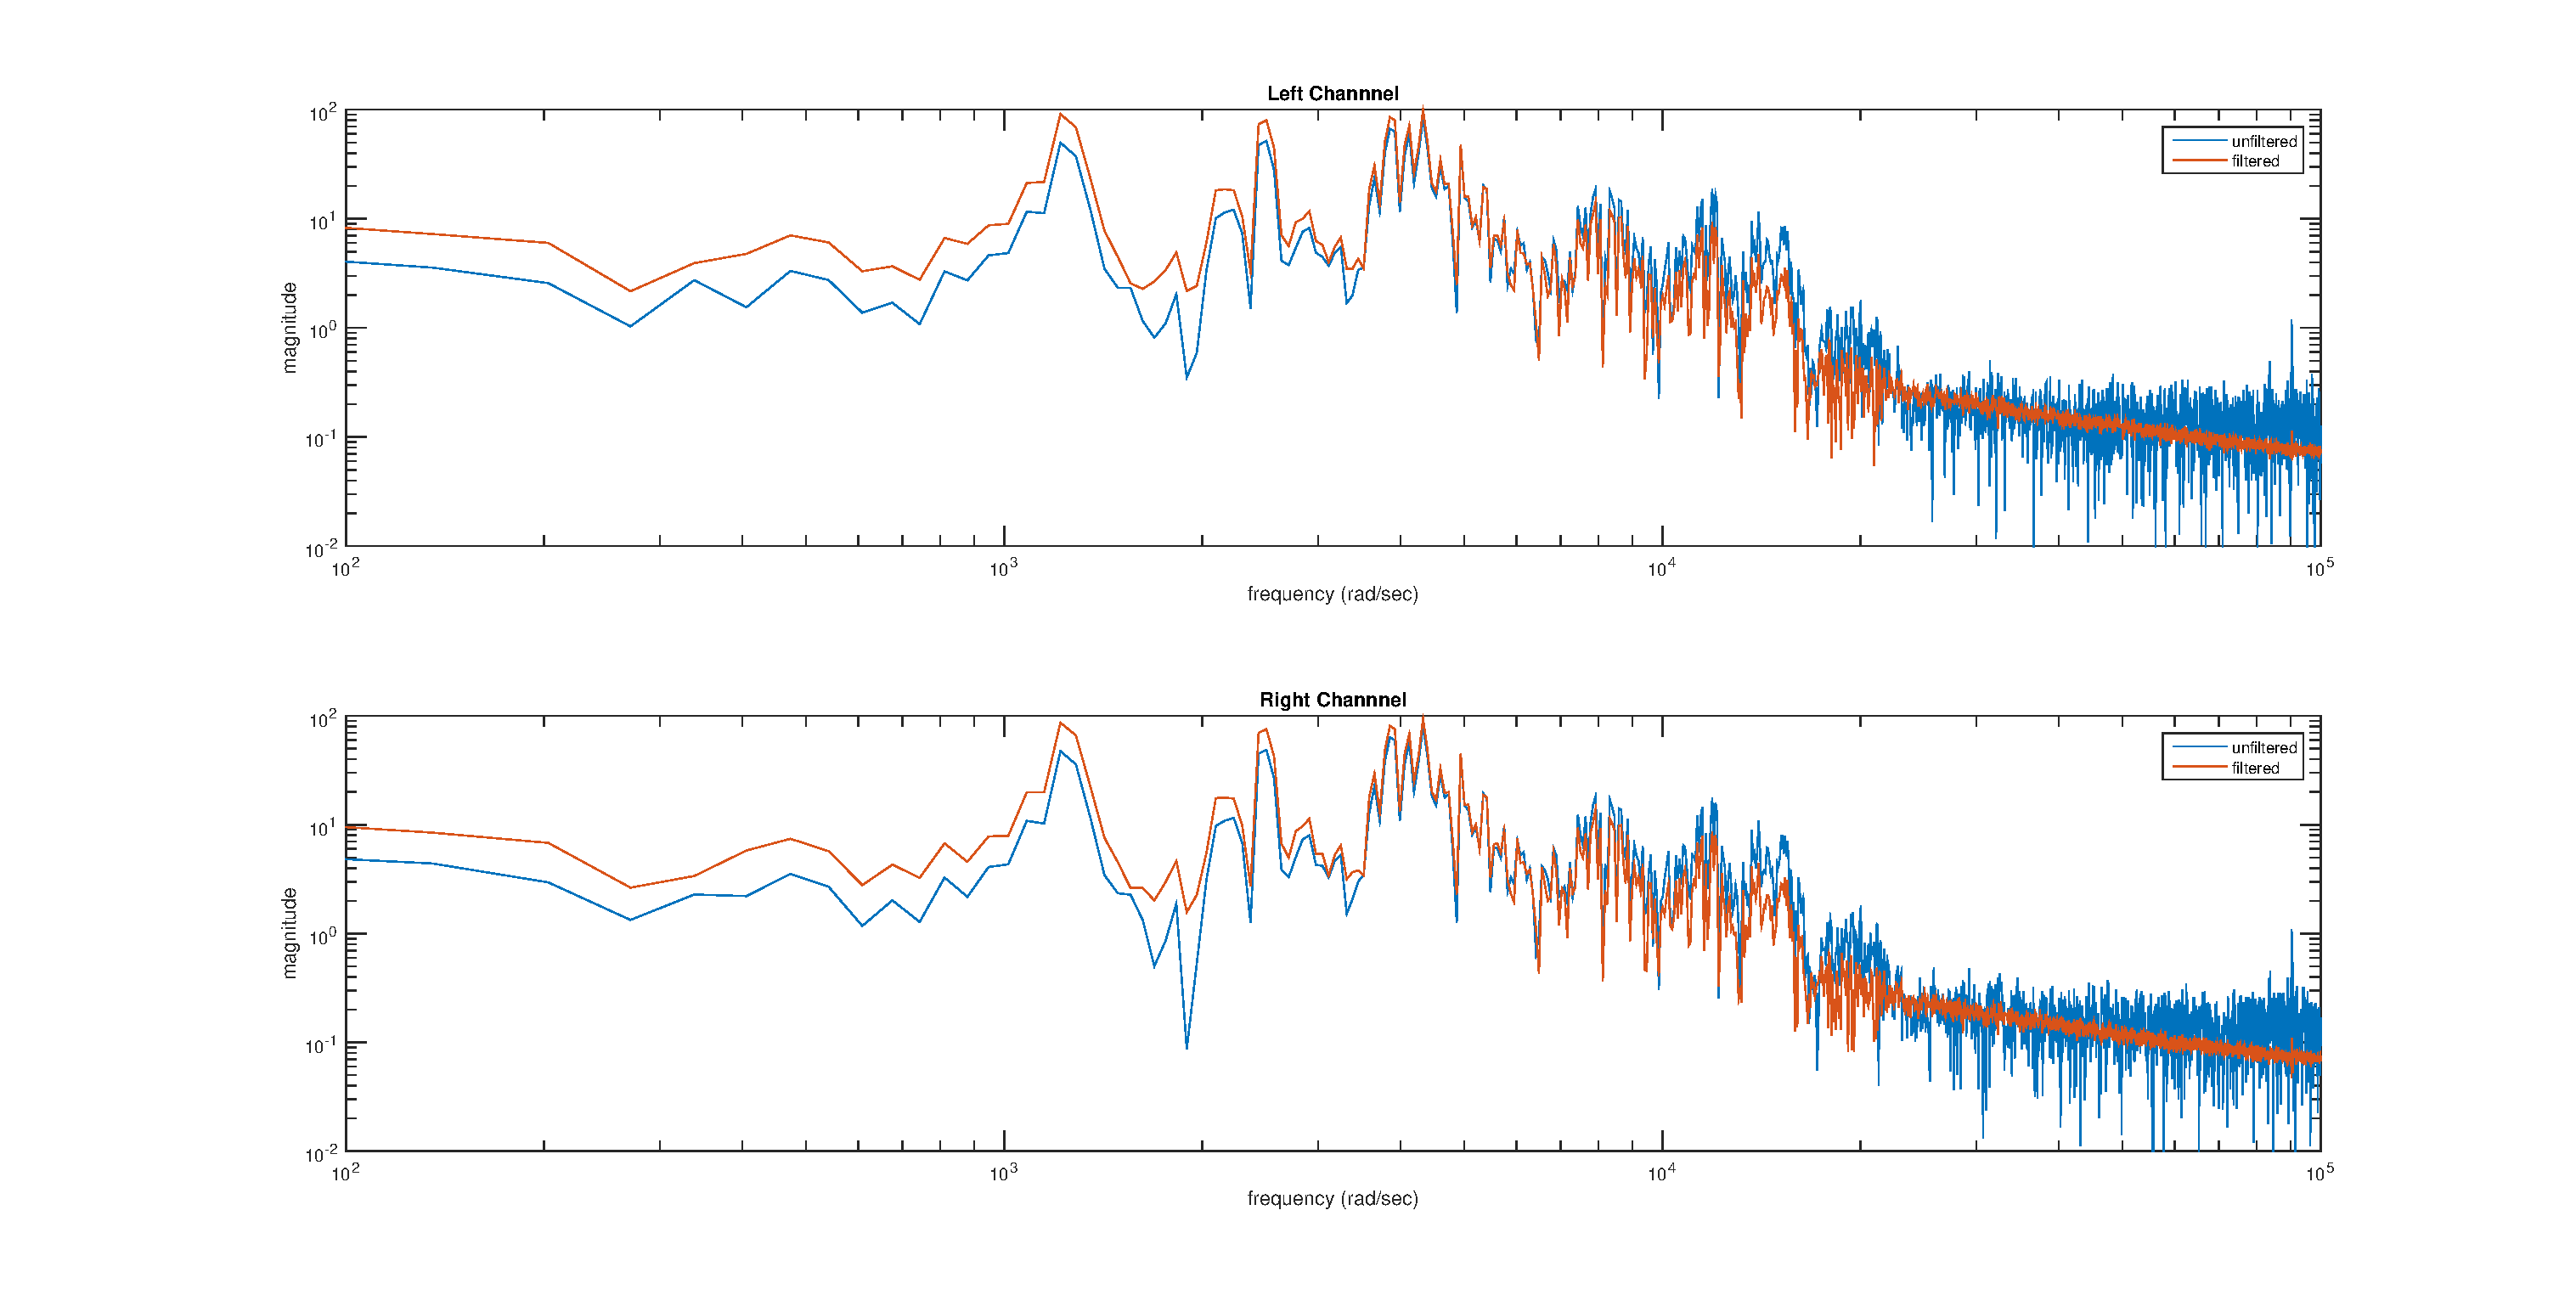
\includegraphics[scale=0.37]{fig4.eps}
	 	\captionof{figure}{Bode plot showing both magnitude in decibels and phase in degrees.}
	 \end{figure}
	
	\newpage
	The code used to implement the FFT and create the plots shown in Figure 4 was appended to the code shown in question 1.1 and question 1.6 and is given below:
	
	\begin{lstlisting}
		% The fft implementation using the number of fft points as 4096
		nfft = 4096;
			
		fft_uleft_sample = fft(sample_uleft,nfft);
		fft_uleft_sample = fft_uleft_sample(1:nfft/2);
		
		fft_uright_sample = fft(sample_uright,nfft);
		fft_uright_sample = fft_uright_sample(1:nfft/2);
		
		fft_yleft_sample = fft(sample_yleft,nfft);
		fft_yleft_sample = fft_yleft_sample(1:nfft/2);
		
		fft_yright_sample = fft(sample_yright,nfft);
		fft_yright_sample = fft_yright_sample(1:nfft/2);
		
		fft_w = (2*pi)*(0:nfft/2-1)*fs/nfft;
		
		% Code plots the samples and the filtered samples from the left 
		% and right channels for the time slice 1.0s to 1.1s
		subplot(2,1,1)
		loglog(fft_w,abs(fft_uleft_sample))
		axis([10^2 10^5 10^-2 10^2]);
		title('Left Channnel')
		xlabel('frequency (rad/sec)')
		ylabel('magnitude')
		hold on
		loglog(fft_w,abs(fft_yleft_sample))
		legend('unfiltered','filtered')
		
		subplot(2,1,2)
		loglog(fft_w,abs(fft_uright_sample))
		axis([10^2 10^5 10^-2 10^2]);
		title('Right Channnel')
		xlabel('frequency (rad/sec)')
		ylabel('magnitude')
		hold on
		loglog(fft_w,abs(fft_yright_sample))
		legend('unfiltered','filtered')
	\end{lstlisting}
\end{document}
